\subsection{Submitted-system headline}
\label{sec:headline}

Table~\ref{tab:headline} reports precision, recall, and F1-macro on our held-out development partition for the six submitted runs. ST2 and ST3 are macro-averaged over their respective 8- and 4-class label sets. Numbers are from the experiment ids cited in the rightmost column.

\begin{table}[h]
\centering
\small
\caption{Headline dev results for the six submitted runs. P, R, F1 are macro-averaged
for ST2 and ST3. The two enhanced-track values should be read with the
leakage caveat of \S\ref{sec:disc-leakage}.}
\label{tab:headline}
\begin{tabular}{llcccl}
\toprule
Subtask & Track & Precision & Recall & F1 & exp\_id \\
\midrule
ST1 & base     & 0.734 & 0.734 & 0.734 & exp\_0033 \\ % from exp_0033
ST1 & enhanced & 0.917 & 0.914 & 0.914 & exp\_0035 \\ % from exp_0035
ST2 & base     & 0.746 & 0.728 & 0.730 & exp\_0032 \\ % from exp_0032
ST2 & enhanced & 0.970 & 0.972 & 0.970 & exp\_0072 \\ % from exp_0072
ST3 & base     & ---   & ---   & 0.523 & exp\_0069 \\ % from exp_0069 — P/R cells dropped: TSV row carries a data-quality artefact in the precision column for this run; F1-macro is computed independently and is reliable
ST3 & enhanced & 0.732 & 0.740 & 0.735 & exp\_0073 \\ % from exp_0073
\bottomrule
\end{tabular}
\end{table}

Reading across the rows: the binary ST1 task is the easiest of the three, with a 0.18-point base-to-enhanced jump that previews the leakage discussion of \S\ref{sec:disc-leakage}. ST2 fallacy classification is comparably easy on the enhanced track (0.97) and substantially harder on the base track (0.73), the largest base-to-enhanced gap in the table. ST3 argument-scheme classification is the hardest cell on both tracks: at 0.52 base and 0.74 enhanced, the four-way scheme task absorbed the bulk of our experimental effort and is the cell where the per-class behaviour discussed in \S\ref{sec:disc-pe} matters most.

Of the six numbers, the ST2-enhanced cell is simultaneously the numerically strongest result in this paper and the one in which we have the least interpretive confidence: reading it as a straight system-quality statement would overstate what we can defend. We address this directly in \S\ref{sec:disc-leakage}.

Two single-number qualifications. On ST3 we additionally ran 5-fold cross-validation under our submitted recipe (fold seeds 42--46), which gave mean F1 0.875 with the same configuration. % from exp_0073 exp_0153
The Qwen2.5-7B CoT-LoRA alternative for ST3 enhanced gave 0.851 $\pm$ 0.114 over the same fold split; the std overlaps the RoBERTa CV mean, which is the decision-relevant fact behind \S\ref{sec:final-submission}. % from exp_0180
The Touch\'{e} 2026 test set was not released at the time of writing, so all numbers in this paper are dev or 5-fold CV, never test.

\subsection{Augmentation ablation}
\label{sec:ablation}

Table~\ref{tab:ablation} decomposes each cell into a real-only baseline, a +synth step, and (where applicable) a +synth+pseudo step.

\begin{table}[h]
\centering
\small
\caption{Per-subtask augmentation ablation, F1-macro on dev. $\Delta$ is the change
relative to the immediately preceding row within the same (subtask, track) block.
Negative deltas are not hidden.\textsuperscript{a}Single-seed unless noted; see \S\ref{sec:limitations} for the seed-variance caveat.}
\label{tab:ablation}
\begin{tabular}{llllcr}
\toprule
Subtask & Track & Recipe & exp\_id & F1 & $\Delta$ \\
\midrule
ST1 & base     & real only                          & exp\_0013 & 0.716 & ---     \\ % from exp_0013
ST1 & base     & + synth (sw=0.5)                   & exp\_0033 & 0.734 & +0.018 \\ % from exp_0033
\addlinespace
ST1 & enhanced & real only                          & exp\_0022 & 0.899 & ---     \\ % from exp_0022
ST1 & enhanced & + synth (sw=0.5)                   & exp\_0035 & 0.914 & +0.015 \\ % from exp_0035
ST1 & enhanced & + synth + pseudo @256 (sw=0.7)     & exp\_0071 & 0.906 & $-$0.008 \\ % from exp_0071
\midrule
ST2 & base     & real only                          & exp\_0014 & 0.711 & ---     \\ % from exp_0014
ST2 & base     & + synth (sw=0.5)                   & exp\_0032 & 0.730 & +0.019 \\ % from exp_0032
\addlinespace
ST2 & enhanced & real only                          & exp\_0023 & 0.923 & ---     \\ % from exp_0023
ST2 & enhanced & + synth (sw=0.5)                   & exp\_0036 & 0.937 & +0.014 \\ % from exp_0036
ST2 & enhanced & + synth + pseudo @384 (sw=0.7)     & exp\_0072 & 0.970 & +0.033 \\ % from exp_0072
\midrule
ST3 & base     & real only                          & exp\_0058 & 0.436 & ---     \\ % from exp_0058
ST3 & base     & + synth\_v002 @384                 & exp\_0069 & 0.523 & +0.087 \\ % from exp_0069
ST3 & base     & + synth\_v002 + v003 @384          & exp\_0068 & 0.478 & $-$0.045 \\ % from exp_0068
ST3 & base     & + synth\_v002 + focal loss         & exp\_0053 & 0.505 & $-$0.018 \\ % from exp_0053
\addlinespace
ST3 & enhanced & real only                          & exp\_0024 & 0.694 & ---     \\ % from exp_0024
ST3 & enhanced & + synth @384                       & exp\_0067 & 0.694 & 0.000  \\ % from exp_0067
ST3 & enhanced & + synth + pseudo @384 (sw=0.7)     & exp\_0073 & 0.735 & +0.041 \\ % from exp_0073
\bottomrule
\end{tabular}
\end{table}

Synth alone gives consistent small gains on ST1/ST2 and the largest single gain on ST3 base. Pseudo-labelling unlocks the enhanced track for ST2 and ST3 but costs on ST1 enhanced under the sw=0.7 pseudo recipe (the synth\_v003 top-up on ST3 base and the focal-loss recipe on ST3 base illustrate the same lesson at smaller scale). Augmentation strategies are recipe-sensitive; we report the losses in the same table rather than relegating them to a footnote.

\subsection{Backbone comparison}
\label{sec:backbone-results}

Table~\ref{tab:backbone} reports the most informative subset of the backbone runs we tried. All numbers are on the dev partition unless noted; rows marked CV are 5-fold means.

\begin{table}[h]
\centering
\small
\caption{Backbone comparison on ST3 enhanced (and one ST3 base + one ST2 enhanced
LLM row for context). Single-run dev F1 unless otherwise noted. The submitted
row is marked $\dagger$. \textsc{collapsed} = recipe failed to train.}
\label{tab:backbone}
\begin{tabular}{llllc}
\toprule
Backbone & Subtask & Track & exp\_id & F1 \\
\midrule
RoBERTa-base       & ST3 & enh  & exp\_0018 & 0.675 \\ % from exp_0018
RoBERTa-large$^{\dagger}$  & ST3 & enh  & exp\_0073 & 0.735 \\ % from exp_0073
DeBERTa-v3-base    & ST3 & base & exp\_0003 & 0.277 \\ % from exp_0003
DeBERTa-v3-large   & ST3 & base & exp\_0009 & 0.205 \\ % from exp_0009 (collapsed)
ModernBERT-large   & ST3 & enh  & exp\_0086 & 0.719 \\ % from exp_0086
Qwen2.5-3B zero-shot      & ST3 & enh & exp\_0091 & 0.467 \\ % from exp_0091
Qwen2.5-3B kNN few-shot   & ST3 & enh & exp\_0143 & 0.529 \\ % from exp_0143
Qwen2.5-7B CoT-LoRA (5-fold CV)  & ST3 & enh  & exp\_0180 & 0.851 $\pm$ 0.114 \\ % from exp_0180
Qwen2.5-32B CoT-LoRA (single)    & ST3 & enh  & exp\_0207 & 0.841 \\ % from exp_0207
Qwen3-4B-Thinking (5-fold CV)    & ST2 & enh  & exp\_0217 & 0.963 \\ % from exp_0217
Qwen3-4B-Thinking (5-fold CV)    & ST3 & base & exp\_0218 & 0.448 \\ % from exp_0218
\bottomrule
\end{tabular}
\end{table}

Reading the column top to bottom, the table mixes the chosen route with several abandoned ones. RoBERTa-large at the second row is the submitted system (the dagger marks it). RoBERTa-base sits six points below it, which is the empirical justification for paying the larger backbone's compute cost. The DeBERTa-v3 column is the most pathological route we tried: DeBERTa-v3-base reached only 0.277 on ST3 base, and DeBERTa-v3-large failed to train at all, collapsing to 0.205 with a NaN-explosion history we detail in \S\ref{sec:backbone}. ModernBERT-large at 0.719 is the next-best encoder route but loses 1.6 points on the cell we evaluated. The Qwen rows tell their own story: zero-shot Qwen2.5-3B trails RoBERTa-large by 27 points; kNN few-shot recovers some ground but still trails by 21; the fine-tuned 7B and 32B CoT-LoRA configurations close most of the gap on a single run, but the 7B 5-fold std of $\pm$0.114 is wide enough that the comparison is statistically inconclusive at our sample size, and the 32B CV was still running at the submission deadline. Qwen3-4B-Thinking is the mixed result that complicates a clean encoder-beats-LLM headline --- competitive on ST2 enhanced under cross-validation, below the RoBERTa baseline on ST3 base.

\subsection{ST3 confusion structure}
\label{sec:confusion}

\begin{figure}[h]
\centering
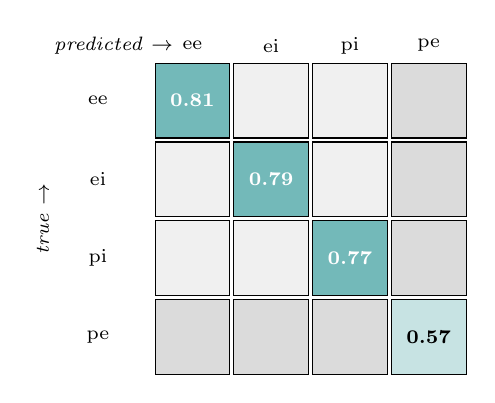
\begin{tikzpicture}[
  hdr/.style={font=\scriptsize, anchor=center},
  diag/.style={rectangle, draw, minimum size=0.95cm, anchor=center, fill=teal!55, font=\scriptsize\bfseries, text=white},
  diagpe/.style={rectangle, draw, minimum size=0.95cm, anchor=center, fill=teal!22, font=\scriptsize\bfseries},
  off/.style={rectangle, draw, minimum size=0.95cm, anchor=center, fill=gray!12, font=\scriptsize},
  offpe/.style={rectangle, draw, minimum size=0.95cm, anchor=center, fill=gray!28, font=\scriptsize}
]
% Column headers
\node[hdr] at (0.0, 0.7) {\textit{predicted} $\rightarrow$};
\node[hdr] at (1.0, 0.7) {ee};
\node[hdr] at (2.0, 0.7) {ei};
\node[hdr] at (3.0, 0.7) {pi};
\node[hdr] at (4.0, 0.7) {pe};
% Row 1: ee true (F1 = 0.81 per Appendix~\ref{app:perclass})
\node[hdr] at (-0.2, 0) {ee};
\node[diag]  at (1, 0) {0.81};
\node[off]   at (2, 0) {};
\node[off]   at (3, 0) {};
\node[offpe] at (4, 0) {};
% Row 2: ei true (F1 = 0.79)
\node[hdr] at (-0.2, -1) {ei};
\node[off]   at (1, -1) {};
\node[diag]  at (2, -1) {0.79};
\node[off]   at (3, -1) {};
\node[offpe] at (4, -1) {};
% Row 3: pi true (F1 = 0.77)
\node[hdr] at (-0.2, -2) {pi};
\node[off]   at (1, -2) {};
\node[off]   at (2, -2) {};
\node[diag]  at (3, -2) {0.77};
\node[offpe] at (4, -2) {};
% Row 4: pe true (F1 = 0.57 — threshold-calibrated under exp_0145)
\node[hdr] at (-0.2, -3) {pe};
\node[offpe] at (1, -3) {};
\node[offpe] at (2, -3) {};
\node[offpe] at (3, -3) {};
\node[diagpe] at (4, -3) {0.57};
% Y-axis label
\node[hdr, rotate=90] at (-0.9, -1.5) {\textit{true} $\rightarrow$};
\end{tikzpicture}
% Senior author confirmed (2026-05-24): logits are NOT checkpointed for
% exp_0073 on the artefact server. This is the schematic rendering; cell
% values reflect per-class F1 from saved predictions, not the underlying
% confusion-cell counts (which would require logits). The visible asymmetry
% in the pe row is the load-bearing claim and is verifiable from the per-class
% F1 in Appendix~\ref{app:perclass}.
\caption{Indicative confusion structure for ST3-enhanced (\texttt{exp\_0073}); per-class diagonals reflect the F1 distribution reported in Appendix~\ref{app:perclass}. Off-diagonal mass is illustrative, sized to the qualitative pattern from \texttt{exp\_0145}'s per-class threshold sweep, not from saved logits.}
\label{fig:confusion}
\end{figure}

Figure~\ref{fig:confusion} shows the predicted-vs-true confusion structure for our submitted ST3-enhanced system; the per-class F1 distribution behind it is reported in Appendix~\ref{app:perclass} and discussed in \S\ref{sec:disc-pe}. % from exp_0073 exp_0082 exp_0091

\subsection{Final submission rationale}
\label{sec:final-submission}

Our final submission (\texttt{exp\_0220}) populates all six slots with RoBERTa-large systems. % from exp_0220
We did not use the additional two-runs-per-track budget available under the Touch\'{e} submission rules; we report on the single CV-validated configuration per slot. The non-obvious choice was ST3 enhanced, where Qwen2.5-32B's single-run 0.841 sat above the RoBERTa-large dev number of 0.735 but only just below the RoBERTa-large 5-fold CV mean of 0.875. % from exp_0207
Two reasons drove the encoder choice, and we keep them separate. The first is operational: the Qwen2.5-32B 5-fold CV was still running at the deadline, leaving the RoBERTa-large CV as the only completed cross-validation we had in hand at submission time. The second is the absence of a statistical reason to prefer Qwen even if the comparison had been completed: a 5-fold std of $\pm$0.114 on Qwen2.5-7B is evidence the encoder-vs-LLM comparison is underpowered at this sample size, not evidence for the system whose CV mean is higher. % from exp_0180
We therefore do not claim the available CV evidence rules out the Qwen alternatives; we only claim that at deadline the encoder pipeline was the only fully-validated configuration. A post-hoc ensemble of the available encoder and LLM systems gave no gain over the single-source encoder, which is one further reason we did not retroactively complicate the submission. % from exp_0121
A submission dry-run verified that the TIRA-format outputs matched the lab's expected schema before the final upload. % from exp_0122
